\documentclass[conference]{IEEEtran}
\IEEEoverridecommandlockouts
\usepackage{cite}
\usepackage{amsmath,amssymb,amsfonts}
\usepackage{algorithmic}
\usepackage{graphicx}
\usepackage{textcomp}
\usepackage{xcolor}
\usepackage{booktabs}
\usepackage{url}
\usepackage{hyperref}
\usepackage{tabularx}
\usepackage{microtype}

\def\BibTeX{{\rm B\kern-.05em{\sc i\kern-.025em b}\kern-.08em
    T\kern-.1667em\lower.7ex\hbox{E}\kern-.125emX}}

\begin{document}

\title{AirSleuth: A Tool-Grounded Domain AI Agent for Explainable $\text{PM}_{2.5}$ Source Attribution and Personalized Activity Decision Support from Public IoT Sensor Networks\\
{\footnotesize \textsuperscript{*}Corresponding Author: Yen-Kai Chen (air.sleuth.project@gmail.com)}
}

\author{\IEEEauthorblockN{Yen-Kai Chen\IEEEauthorrefmark{1}, Hong-Yu Chen\IEEEauthorrefmark{1}, Ting-Chang Wang\IEEEauthorrefmark{1}, Chia-Feng Li\IEEEauthorrefmark{1}, and Sheng-Ru Chou\IEEEauthorrefmark{1}}
\IEEEauthorblockA{\IEEEauthorrefmark{1}Department of Computer Science and Information Engineering / IoT Smart City Research Lab\\
National Taiwan University of Science and Technology / Partner Universities, Taipei, Taiwan\\
Project Repository: \url{https://github.com/A0966411725-png/AirSleuth}}
}

\maketitle

\begin{abstract}
\textbf{(A) Attention Getter / Area:} Ambient fine particulate matter ($\text{PM}_{2.5}$) remains the paramount environmental risk factor, responsible for an estimated 7.9 million premature deaths globally in 2023. While Taiwan recently tightened its national ambient standards and deployed over 10,200 public IoT micro-sensors, existing air-quality services report only a broad, color-coded Air Quality Index (AQI), creating an information paradox where dense measurements fail to yield actionable guidance.
\textbf{(B) Bottleneck / Problem:} In practice, citizens critically need answers to three questions that conventional portals cannot address: (1) \textit{Why} is $\text{PM}_{2.5}$ elevated (hyper-local emission versus regional transboundary plume)?; (2) \textit{How} should individuals adapt (personal activity, duration, and vulnerable subgroup tradeoffs)?; and (3) \textit{Is} the sensor reading credible? Dense low-cost sensors exhibit severe hygroscopic swelling and systematic over-estimation under high relative humidity, and generative large language models (LLMs) notoriously hallucinate numeric environmental metrics.
\textbf{(C) Cure / Core Solution:} We propose \textbf{AirSleuth}, a tool-grounded domain AI agent combining generative language reasoning with deterministic execution. By strictly confining the LLM to user query comprehension, multi-step orchestration, and conversational explanation, all computations---sensor quality control, localized calibration, multi-scale spatial attribution, and action optimization---are delegated to deterministic, logged tools.
\textbf{(D) Development / Methodology:} AirSleuth incorporates: (i) an automated 5-flag data quality pipeline; (ii) city-specific dynamic humidity correction anchored to reference stations; (iii) a multi-scale spatial decomposition algorithm analyzing local excess ($E$) and neighborhood coherence ($C$) across 2, 8, and 15~km radiuses; (iv) an explainable multiple linear regression forecasting module; and (v) an automated number-traceability guardrail that rejects responses containing unverified figures.
\textbf{(E) Experiments / Evaluation:} Evaluated across 15.5 million 5-minute records from 2,560 sensors, 18 reference stations, and 124 weather stations in Taichung and Kaohsiung, 880 semi-synthetic plume injection scenarios, and a 40-question comprehensive Chinese scenario benchmark, AirSleuth achieves an attribution accuracy of 84.0\% (macro-$F_1$ 0.80), accurately rejecting 99.0\% of single-sensor faults.
\textbf{(F) Findings / Impact:} AirSleuth achieves 100\% numeric traceability (0.00 hallucination rate) and 96.0\% behavioral recommendation alignment, compared to 25.0\%--33.0\% for standalone LLMs. All architectural specifications, workflows, and test benches are structured via OpenSpec for full reproducibility.
\end{abstract}

\begin{IEEEkeywords}
Air Quality, $\text{PM}_{2.5}$, Internet of Things (IoT), Low-Cost Sensors, LLM Agent, Tool Use, Model Context Protocol, Spatial Attribution, Spec-Driven Development.
\end{IEEEkeywords}

\section{Introduction}
\IEEEPARstart{A}{mbient} fine particulate matter ($\text{PM}_{2.5}$) represents the single largest environmental risk to public health worldwide, responsible for an estimated 7.9 million premature deaths globally in 2023~\cite{s_060}. In response to accumulating epidemiological evidence demonstrating that cardiovascular and pulmonary toxicity occurs even at very low exposure levels with no identifiable safe threshold~\cite{s_020, s_021}, Taiwan tightened its national ambient air quality standards in 2024 to 12~$\mu\text{g/m}^3$ for annual average and 30~$\mu\text{g/m}^3$ for daily average, concurrently deploying a revised Air Quality Index (AQI) framework~\cite{s_016}. Nevertheless, widespread public health communication remains fundamentally detached from human decision-making: conventional public dashboards reduce intricate spatio-temporal atmospheric dynamics into coarse, city-wide color tiers and generic group-level advisories~\cite{s_032}. Consequently, a systematic review revealed that a median of only 31\% of individuals actively adjust their outdoor activities when air quality deteriorates, citing incomprehensible index scales and lack of actionable, personalized alternatives as primary behavioral barriers~\cite{s_028}.

The proliferation of Internet of Things (IoT) technologies provides an unprecedented opportunity to bridge this gap. Under its national smart city and Civil IoT initiatives, Taiwan deployed more than 10,200 low-cost optical $\text{PM}_{2.5}$ sensors nationwide~\cite{s_013}, streaming real-time measurements at 5-minute intervals via open SensorThings APIs~\cite{s_001}. This dense spatial mesh offers spatial resolution that sparse national reference stations (which average 10--20~km apart) inherently cannot provide. Crucially, dense spatial sensing can distinguish whether a localized elevation is confined to a 2~km radius (e.g., street-level construction or agricultural burning) or represents a 15~km regional stagnation episode. This distinction is of vital practical importance: for a hyper-local event, an individual can successfully avoid exposure simply by relocating several kilometers away; conversely, during a regional air pollution episode, spatial relocation within the city is entirely ineffective, necessitating temporal postponement, indoor relocation, or active air filtration.

Despite this rich IoT infrastructure, three fundamental bottlenecks prevent raw public sensing data from supporting trustworthy personal decisions:
\begin{enumerate}
    \item \textbf{Sensor Bias and Hygroscopic Distortion:} Low-cost optical sensors rely on light scattering, systematically over-estimating true mass concentration by approximately 40\% due to particle hygroscopic swelling under high relative humidity ($\text{RH} > 70\%$)~\cite{s_008, s_009}. Furthermore, empirical calibration functions are strictly site-specific and non-transferable across geographic areas~\cite{s_010, s_058}.
    \item \textbf{Spatial Attribution Ambiguity:} Separating localized plume emissions from broad background regional transport remains a severe challenge; raw spatial nearest-neighbor approaches are notoriously susceptible to isolated sensor defects, false spikes, and localized micro-climate drift~\cite{s_057}.
    \item \textbf{Generative Hallucination and Traceability Void in LLMs:} While Large Language Models (LLMs) excel at natural language reasoning and conversational dialogue, general-purpose LLMs frequently hallucinate numerical metrics and cannot perform physical spatio-temporal calculations~\cite{s_035}. Recent multi-agent architectures (e.g., Neuro-Air~\cite{s_053}) focus primarily on expert environmental scientists querying clean reference stations, failing to address the noise, bias, and uncertainty inherent in citizen-facing IoT streams~\cite{s_055}.
\end{enumerate}

To overcome these barriers, this paper presents \textbf{AirSleuth}, an open-source, tool-grounded domain AI agent engineered for explainable $\text{PM}_{2.5}$ source attribution and personalized activity decision support. AirSleuth enforces an architectural separation of concerns: generative LLMs are strictly confined to semantic question parsing, high-level task planning, and empathic natural language explanation, whereas all empirical calculations, data validation, localized calibration, spatial morphology attribution, and health decision scoring are executed by deterministic, logged programmatic tools.

The primary contributions of this paper are summarized as follows:
\begin{itemize}
    \item \textbf{Tool-Grounded Agent Architecture with Number-Traceability Guardrails:} We formulate an end-to-end domain agent utilizing function calling and tool contracts (inspired by the Model Context Protocol) coupled with an automated post-generation regex verification engine that strictly rejects and rewrites any response containing numerical tokens absent from deterministic tool logs.
    \item \textbf{Multi-Scale Spatial Attribution Methodology:} We introduce a multi-tier spatial morphology algorithm operating over 2~km, 8~km, and 15~km neighborhood radiuses to robustly decompose sensor measurements into local excess ($E$) and spatial coherence ($C$), systematically differentiating hyper-local sources, subregional clusters, regional plumes, and single-sensor anomalies.
    \item \textbf{Empirical Validation on Massive Real-World IoT Datasets:} We validate the system against 15.5 million 5-minute records across 2,560 micro-sensors, 18 national monitoring stations, and 124 weather stations in Taichung and Kaohsiung, supported by 880 semi-synthetic injection trials and a 40-scenario benchmark.
    \item \textbf{Open-Source Spec-Driven Development Workflow:} We provide an open-source implementation governed by OpenSpec, bridging architectural design documents directly to executable specifications, regression suites, and live interactive dashboards.
\end{itemize}

\section{Related Work}
Existing research relevant to intelligent environmental sensing spans four primary domains: LLM agents for data science, low-cost sensor calibration, spatial source separation, and environmental health risk communication.

\subsection{LLM Agents and Deterministic Tool Augmentation}
Recent advances in Large Language Models (LLMs) have demonstrated remarkable efficacy in orchestrating complex problem-solving workflows via the ReAct (Reasoning and Acting) paradigm~\cite{s_035}. In the environmental and atmospheric sciences, domain-specific multi-agent systems have emerged to automate data retrieval and reporting. For instance, Neuro-Air~\cite{s_053} coordinates five collaborative sub-agents to inspect national air monitoring data, achieving 88.4\% operational accuracy on verifiable scientific queries. Similarly, specialized agentic workflows have been applied to analyze wildfire events~\cite{s_054}, interface with sensors via the Model Context Protocol (MCP)~\cite{s_036}, or synthesize Python analytical scripts directly from natural language prompts~\cite{s_037}. 

However, a comprehensive survey across 45 data-centric LLM agents revealed that over 90\% lack explicit verification, safety constraints, or numerical traceability mechanisms~\cite{s_055}. More critically, existing systems uniformly assume clean, trustworthy input data sourced from certified, sparse government reference stations. When deployed in citizen-facing contexts over tens of thousands of noisy, uncalibrated consumer IoT nodes, standard agentic architectures suffer catastrophic failure: they accept biased sensor readings uncritically, propagate false alarms from broken nodes, and frequently hallucinate plausible-sounding yet fabricated exposure numbers~\cite{s_035}. AirSleuth resolves this vulnerability by establishing a deterministic execution perimeter where every numeric claim is mathematically derived from logged tool calls.

\subsection{Low-Cost Sensor Calibration and Physical Distortions}
Low-cost particulate matter sensors (such as optical particle counters utilizing Mie scattering) offer spatial granularity but suffer from severe physical inaccuracies. Extensive evaluations in the United States demonstrated that raw optical sensors systematically overestimate $\text{PM}_{2.5}$ mass concentrations by 40\%--50\% due to hygroscopic aerosol growth, exhibiting highly non-linear distortion once relative humidity exceeds 70\%~\cite{s_008, s_009}. 

To correct these errors, diverse regression and machine learning algorithms---ranging from multiple linear regression (MLR) to random forests and gradient boosted trees---have been proposed~\cite{s_011, s_041}. However, environmental calibration models are notoriously non-transferable across spatial and seasonal domains~\cite{s_010}. In Taiwan, empirical analyses revealed that a single nationwide calibration formula fails completely across varying climatic zones, demanding spatially varying coefficient models~\cite{s_058}. Crucially, previous calibration literature treats sensor correction as an isolated offline preprocessing task, completely disconnected from user-facing decision workflows. AirSleuth integrates dynamic, city-specific calibration into the agent's real-time reasoning loop, substituting faulty on-board sensor hygrometers with validated nearby meteorological stations.

\subsection{Spatial Source Attribution: Local vs. Regional Plumes}
Determining whether an observed pollution spike arises from a localized emission source or a widespread regional transport event is vital for both enforcement and public guidance. Established spatial analysis techniques include spatial moving medians, peak identification filters, background normalization, and spectral frequency filtering~\cite{s_045, s_047}. Nonetheless, comparative studies demonstrate that no single method universally dominates across diverse geographic topographies~\cite{s_057}.

Moreover, naive spatial approaches, such as relying on the single nearest sensor, are highly vulnerable to sensor drift, localized non-representative obstructions (e.g., incense burning or vehicle exhaust directly adjacent to the inlet), and transient device faults. AirSleuth overcomes this vulnerability through a multi-tier spatial decomposition framework. By computing median background baselines ($B$) across 15~km, local medians ($L$) across 2~km, and evaluating neighborhood elevation coherence ($C$), AirSleuth isolates true local point plumes from regional meteorological inversions while rejecting single-sensor anomalies.

\subsection{Personalized Exposure Assessment and Activity Guidance}
Public health advisories have historically relied on threshold-based color charts (e.g., Green/Yellow/Red bands) tied exclusively to outdoor ambient concentrations. However, epidemiological and human activity studies consistently demonstrate that \textit{ambient concentration does not equal personal exposure}~\cite{s_034}. The National Human Activity Pattern Survey (NHAPS) confirmed that urban residents spend over 87\% of their daily time indoors, where indoor infiltration and filtration drastically alter true inhaled dose~\cite{s_034}. Furthermore, physical exercise drastically elevates ventilation rates, creating a complex biological tradeoff: in clean to moderate air ($\text{PM}_{2.5} < 25~\mu\text{g/m}^3$), the cardiovascular benefits of physical activity significantly outweigh the minor pollution risks, whereas at higher concentrations the protective mortality benefit diminishes from 30\% down to 12\%--15\%~\cite{s_033, s_061}.

Existing portals offer binary ``go / do not go'' warnings that ignore activity duration, route alternatives, and biological vulnerability, resulting in pervasive public non-compliance~\cite{s_028}. AirSleuth transforms health advice from a prohibitive ban into an evidence-based multi-objective optimization problem, dynamically ranking schedule shifts, spatial detours, intensity modulations, and indoor substitutions.

\begin{table*}[t]
\caption{Systematic Comparison of Air Quality Information Paradigms}
\label{tab:comparison}
\centering
\begin{tabularx}{\textwidth}{lXXXX}
\toprule
\textbf{Evaluation Dimension} & \textbf{Traditional AQI Portals} & \textbf{Standalone LLMs (e.g., ChatGPT)} & \textbf{Expert Data Agents (e.g., Neuro-Air)} & \textbf{AirSleuth (This Work)} \\
\midrule
\textbf{Target Audience} & General public (passive) & General conversational users & Environmental scientists / analysts & Citizens, athletes, vulnerable groups \\
\textbf{Primary Data Source} & Sparse certified stations & Static pre-training corpora & Certified reference stations & Dense IoT sensors (10,000+) + Stations \\
\textbf{Sensor Quality Control} & Pre-screened by EPA staff & None (data unaware) & Assumes clean reference data & Automated 5-flag deterministic pipeline \\
\textbf{Dynamic Calibration} & N/A (certified instruments) & None & None & City-specific, weather-anchored MLR \\
\textbf{Spatial Attribution} & Coarse administrative zone & Qualitative hallucination & Python script generation & Multi-scale (2/8/15 km) coherence metric \\
\textbf{Numeric Traceability} & Static display table & Fails (hallucinates values) & Unconstrained code execution & Strict regex guardrail \& replay logs \\
\textbf{Action Guidance} & Coarse demographic warnings & Generic wellness advice & None (data reporting only) & Multi-attribute personalized ranking \\
\textbf{Development Paradigm} & Monolithic web service & Monolithic LLM prompt & Ad-hoc agent prompts & OpenSpec Spec-Driven Development \\
\bottomrule
\end{tabularx}
\end{table*}

\section{System Architecture and Implementation}

\subsection{Architectural Overview}
AirSleuth is structured into eight modular components (Fig.~\ref{fig:arch}), enforcing an uncompromising boundary between stochastic language generation and deterministic scientific computing:
\begin{enumerate}
    \item \textbf{User Persona Module ($\mathcal{M}_1$):} Contextualizes user parameters including geographical coordinates, activity duration, metabolic intensity (resting, walking, vigorous running), and biological vulnerability (general vs. sensitive: pediatric, geriatric, asthmatic).
    \item \textbf{Query Parser Module ($\mathcal{M}_2$):} Extracts spatial landmarks (mapped to WGS84 coordinates across 67 Taiwanese administrative districts), temporal target windows, and activity constraints.
    \item \textbf{Planner Agent ($\mathcal{M}_3$):} Powered by Gemini 3.5 Flash-Lite, operating via ReAct function calling across clean tool contracts.
    \item \textbf{Data Ingestion \& QC ($\mathcal{M}_4$):} Ingests 5-minute SensorThings IoT streams, hourly national stations, and meteorological data, tagging each record with quality flags.
    \item \textbf{Analytics Engine ($\mathcal{M}_5$):} Computes spatial metrics ($B, L, E, C$), applies localized calibration, and generates short-term trend forecasts.
    \item \textbf{Domain Knowledge Repository ($\mathcal{M}_6$):} Structures peer-reviewed epidemiological rules, official 2025 AQI break-points, and activity tradeoff formulations.
    \item \textbf{Personalized Decision Module ($\mathcal{M}_7$):} Computes inhalation exposure doses and ranks candidate behavioral adaptations.
    \item \textbf{Output Formatter \& Traceability Verifier ($\mathcal{M}_8$):} Renders responses into a mandatory 4-part structure (\textit{Conclusion, Underlying Cause, Concrete Action, Confidence Level}) and rejects unverified numerical claims.
\end{enumerate}

\begin{figure}[t]
\centering
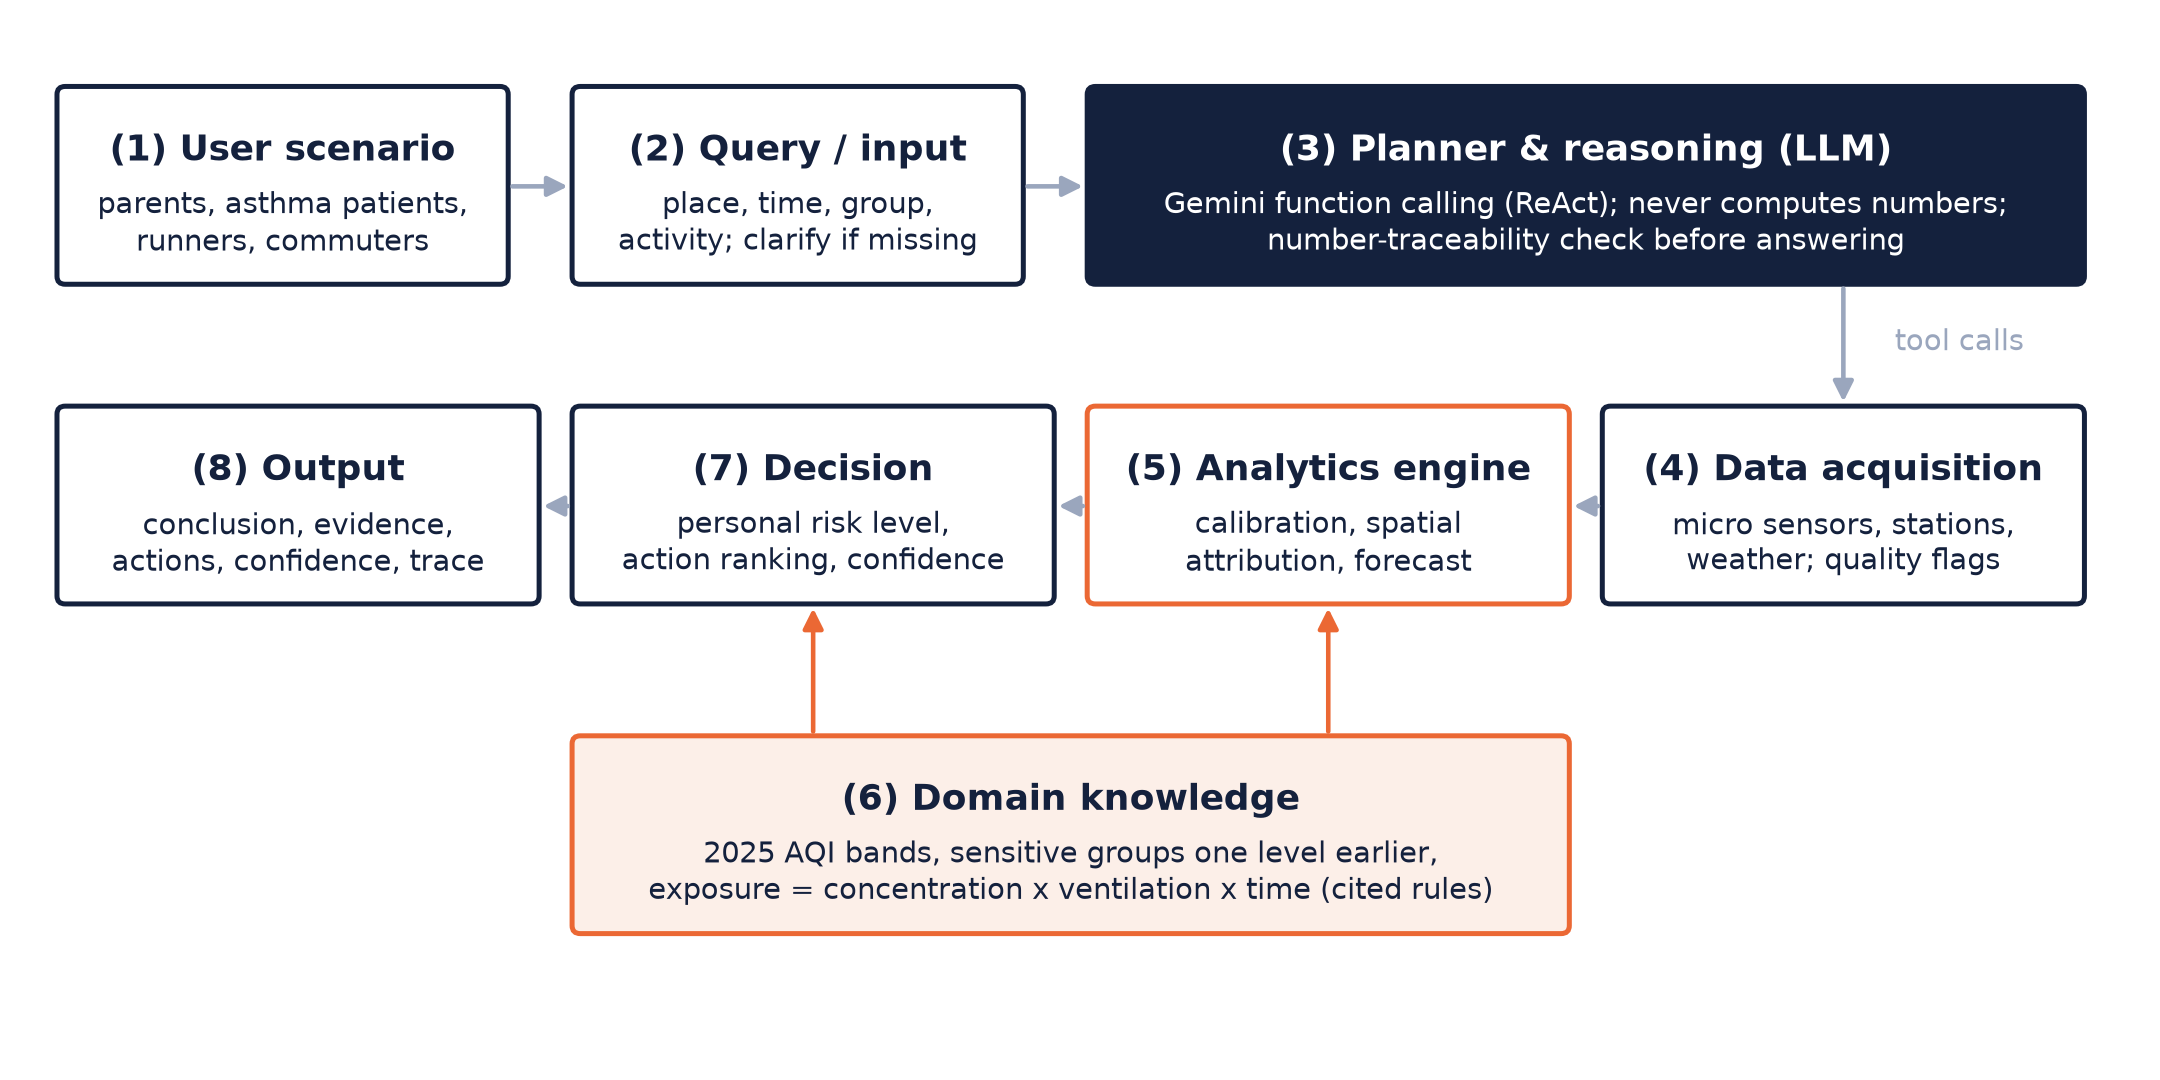
\includegraphics[width=\columnwidth]{figures/fig1_architecture.png}
\caption{AirSleuth end-to-end system architecture. Generative LLMs are confined to reasoning and synthesis, while deterministic tools execute all scientific calculations.}
\label{fig:arch}
\end{figure}

\subsection{Data Quality Control and Environmental Anchoring}
Raw sensor readings undergo an automated quality assessment pipeline:
\begin{equation}
\text{Flag}(s) \in \{\text{Valid}, \text{Missing}, \text{Negative}, \text{Extreme}, \text{Stuck}, \text{RH\_Invalid}\}
\end{equation}
where $\text{Extreme}$ denotes $\text{PM}_{2.5} > 500~\mu\text{g/m}^3$, $\text{Stuck}$ denotes identical measurements across 12 consecutive 5-minute intervals (1 hour), and $\text{RH\_Invalid}$ flags non-physical humidity readings ($<0\%$ or $>100\%$). In Taichung, empirical audits revealed that 28\% of sensor transmissions report exactly $\text{RH} = 0\%$. AirSleuth preserves the particle reading while anchoring the calibration module to the nearest automatic meteorological station.

\subsection{Multi-Scale Spatial Attribution Algorithm}
To classify whether pollution is localized or regional, AirSleuth defines three concentric spatial zones around query coordinate $(x, y)$: local radius $R_{\text{loc}} = 2$~km (doubled up to 8~km if valid sensor count $N < 5$), subregional radius $R_{\text{sub}} = 8$~km, and regional radius $R_{\text{reg}} = 15$~km. 

Let $B$ be the spatial median across all usable sensors within $R_{\text{reg}}$, and $L$ be the median within $R_{\text{loc}}$. The local excess is computed as $E = L - B$. A sensor $s_i$ is classified as \textit{rising} if its current concentration exceeds its preceding 6-hour median by at least 50\% \textit{and} by an absolute margin of at least $5~\mu\text{g/m}^3$:
\begin{equation}
\text{Rising}(s_i) = \left( s_i(t) > 1.5 \cdot \text{Med}_{t-6h}(s_i) \right) \land \left( s_i(t) - \text{Med}_{t-6h}(s_i) \ge 5 \right)
\end{equation}
The absolute term $5~\mu\text{g/m}^3$ is critical: in pristine air (e.g., $4~\mu\text{g/m}^3$ rising to $6.5~\mu\text{g/m}^3$), percentage-only thresholds falsely trigger alarm states due to sensor quantization noise. Spatial coherence ratios $C$, $C_{\text{sub}}$, and $C_{\text{ring}}$ denote the proportion of rising sensors within 15~km, within 8~km, and in the annular ring between 8 and 15~km, respectively. Source attribution follows a deterministic decision hierarchy:
\begin{itemize}
    \item \textbf{Regional Episode:} $C \ge 0.6 \land E < \max(5, 0.3 \cdot B)$
    \item \textbf{Subregional Cluster:} $C < 0.6 \land C_{\text{sub}} \ge 0.3 \land C_{\text{ring}} < 0.3 \land N_{\text{sub}} \ge 5$
    \item \textbf{Local Emission Source:} $E \ge \max(10, 0.5 \cdot B) \land C < 0.3 \land N_{\text{rising, local}} \ge 2$
    \item \textbf{Suspected Sensor Fault:} $E \ge 10 \land N_{\text{rising, local}} < 2$ (isolated spike)
    \item \textbf{Mixed Episode:} $C \ge 0.6 \land E \ge \max(10, 0.5 \cdot B)$
    \item \textbf{No Clear Event:} Default baseline.
\end{itemize}

\subsection{Number-Traceability Guardrail}
To eliminate LLM hallucination, the Output Formatter ($\mathcal{M}_8$) parses the agent's draft response with strict regular expressions matching any numerical quantity bound to physical units ($\mu\text{g/m}^3$, \%, km, m/s, hours). Every detected numeric scalar $v_{\text{draft}}$ must satisfy:
\begin{equation}
\exists v_{\text{log}} \in \mathcal{V}_{\text{tools}} \quad \text{s.t.} \quad |v_{\text{draft}} - v_{\text{log}}| \le \epsilon
\end{equation}
where $\epsilon$ accounts for display rounding ($\pm 0.5$ unit). If an unverified number is discovered, the response is discarded, the LLM is prompted with the discrepancy to regenerate, and persistent failure immediately triggers fallback to a deterministic template.

\section{Experimental Setup and Empirical Results}

\subsection{Data Corpus and Benchmarking Suite}
Experiments were conducted using 15.5 million 5-minute records gathered from 2,560 Civil IoT sensors across Taichung (1,191 sensors) and Kaohsiung (1,369 sensors) between October and November 2026, paired with 18 national monitoring stations and 124 weather stations.

The evaluation protocol encompasses four distinct benchmarks:
\begin{itemize}
    \item \textbf{E1: Forecasting Accuracy:} Evaluating 1-h, 3-h, and 6-h ahead forecasts using persistence, Multiple Linear Regression (MLR), Random Forests, and Gradient Boosted Trees.
    \item \textbf{E2: Sensor Calibration:} Leave-one-site-out cross-validation against certified reference stations.
    \item \textbf{E3: Spatial Attribution under Semi-Synthetic Injections:} 880 controlled injection scenarios across clean atmospheric baselines ($<5\%$ sensors rising), testing detection of local ($+10/15/25~\mu\text{g/m}^3$), subregional ($+8/12/20~\mu\text{g/m}^3$), regional ($+8/12/20~\mu\text{g/m}^3$ across 15~km), and isolated sensor faults ($+40~\mu\text{g/m}^3$ single node).
    \item \textbf{E4: End-to-End Agent Benchmark:} 40 complex Traditional Chinese prompts across 6 real historical episodes, testing 4 architectural designs: AQI-only rule engine, LLM-only (unaugmented), LLM with raw uncurated tools, and AirSleuth.
\end{itemize}

\begin{figure*}[t]
\centering
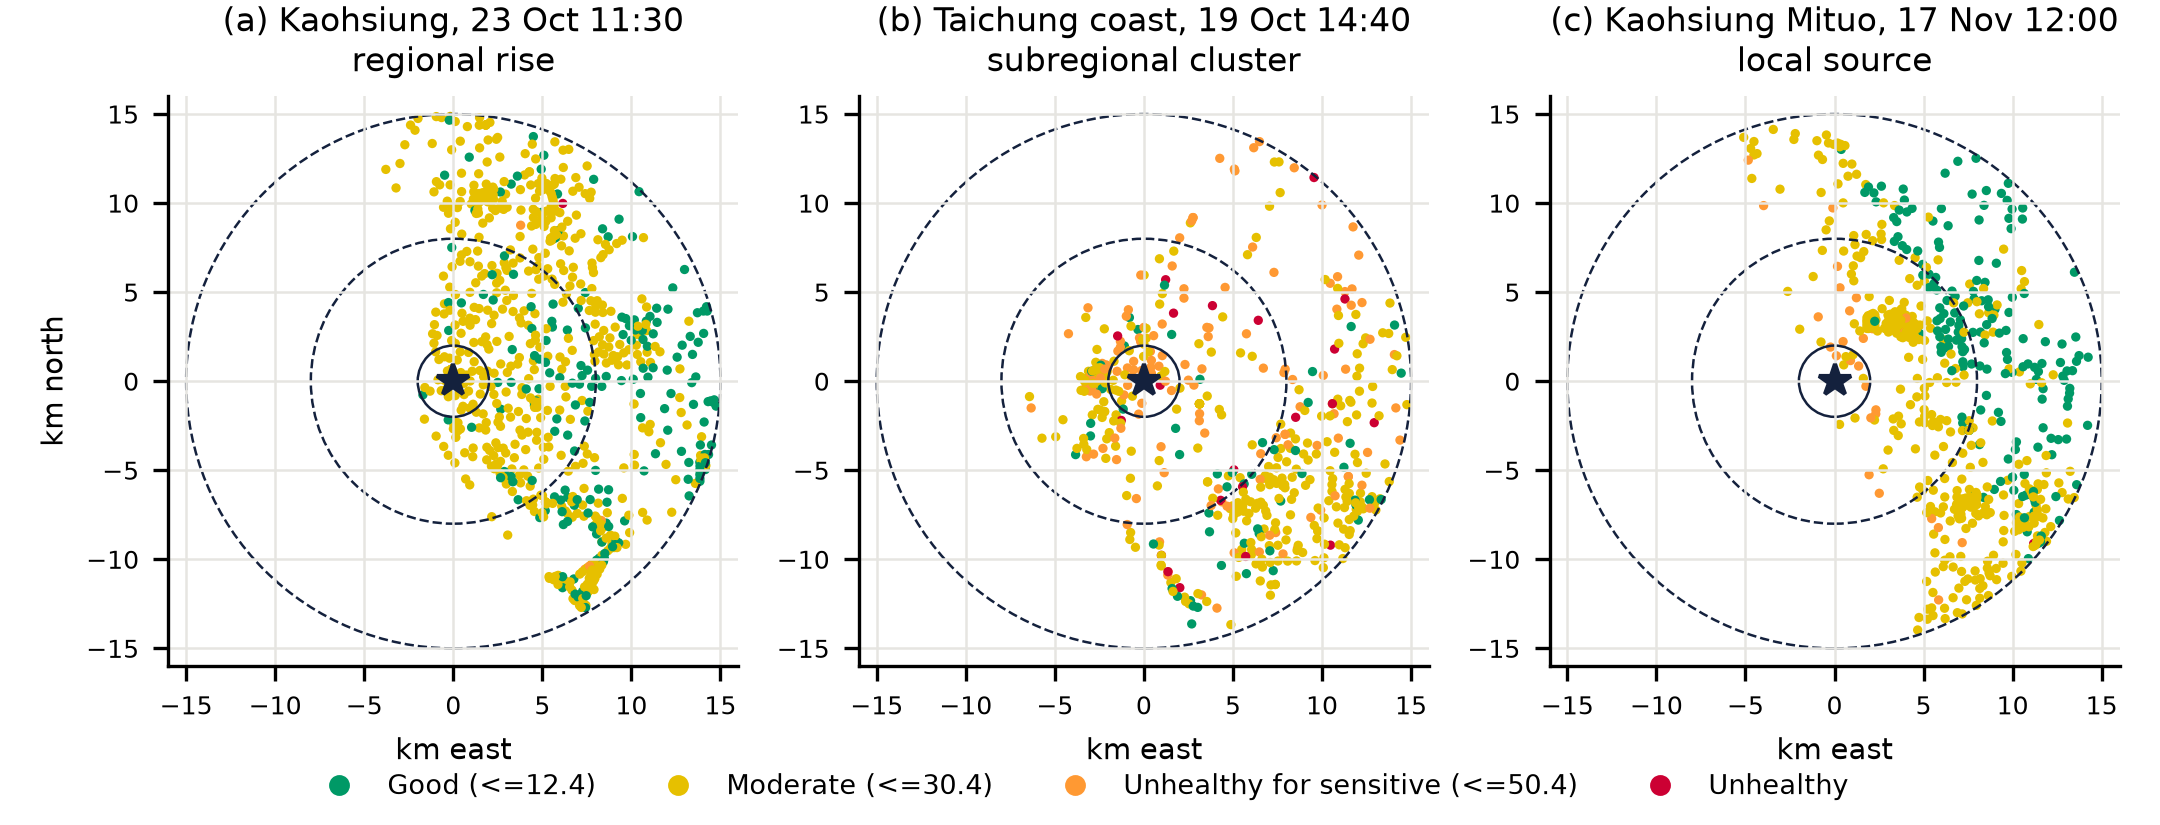
\includegraphics[width=0.95\textwidth]{figures/fig2_cases.png}
\caption{Spatial attribution across three real-world pollution episodes in Taiwan: (a) Kaohsiung regional event (23 Oct 2026, $C = 0.90$); (b) Taichung coastal subregional cluster (19 Oct 2026, $C_{\text{sub}} = 0.38$); (c) Kaohsiung Mituo hyper-local plume (17 Nov 2026, $E = 14.3~\mu\text{g/m}^3$).}
\label{fig:cases}
\end{figure*}

\subsection{Experimental Results}

\subsubsection{Forecasting and Calibration (E1, E2)}
As documented in Table~\ref{tab:results_forecast}, gradient boosted trees achieved the lowest Mean Absolute Error (MAE) at 6 hours (4.74~$\mu\text{g/m}^3$), representing a 17\% improvement over persistence. However, MLR achieved a comparable MAE of 4.97~$\mu\text{g/m}^3$ while providing fully inspectable and explainable linear coefficients. AirSleuth maintains MLR in production to ensure transparency. In calibration, introducing meteorological relative humidity ($\text{RH}$) reduced MAE in Taichung from 4.07 to 3.24~$\mu\text{g/m}^3$, successfully correcting the severe hygroscopic over-estimation observed during high-humidity periods ($\text{RH} \ge 90\%$).

\begin{table}[h]
\caption{E1 Forecast Error and E2 Calibration Performance}
\label{tab:results_forecast}
\centering
\begin{tabular}{lcccc}
\toprule
\textbf{Metric / Task} & \textbf{Persistence} & \textbf{MLR} & \textbf{Best ML} \\
\midrule
E1 1-h Forecast MAE ($\mu\text{g/m}^3$) & 3.35 & 3.19 & 3.16 \\
E1 3-h Forecast MAE ($\mu\text{g/m}^3$) & 4.60 & 4.29 & 4.10 \\
E1 6-h Forecast MAE ($\mu\text{g/m}^3$) & 5.69 & 4.97 & 4.74 \\
E1 6-h AQI-Band Hit Rate & 0.67 & 0.71 & 0.72 \\
\midrule
E2 Calibration Taichung MAE & 4.07 (raw) & 3.36 (lin) & 3.24 (+RH) \\
E2 Calibration Kaohsiung MAE & 3.52 (raw) & 3.02 (lin) & 3.02 (lin) \\
\bottomrule
\end{tabular}
\end{table}

\subsubsection{Spatial Source Attribution Performance (E3)}
On the 880 semi-synthetic injection trials (Table~\ref{tab:attribution}), AirSleuth achieves an overall classification accuracy of 84.0\% and a macro-$F_1$ score of 0.80. In contrast, the conventional AQI-only rule completely fails to recognize localized plumes, categorizing any elevated reading as an undifferentiated regional alert. The nearest-sensor heuristic exhibits severe fragility: while it detects local plumes, it misclassifies 100\% of single-sensor hardware faults as active local pollution sources. AirSleuth limits fault false alarms to just 1.0\% because median pooling effectively filters out isolated anomalies. Ablation of the 8~km subregional tier causes subregional recall to drop from 88.0\% to 0.0\%, demonstrating the necessity of the multi-scale spatial design.

\begin{table}[h]
\caption{E3 Spatial Attribution Evaluation on 880 Injected Cases}
\label{tab:attribution}
\centering
\begin{tabular}{lcccc}
\toprule
\textbf{Architecture / Rule} & \textbf{Accuracy} & \textbf{Macro-$F_1$} & \textbf{Fault as Local} & \textbf{Subreg. Recall} \\
\midrule
AQI-Only Baseline & 24.1\% & 0.12 & 0.0\% & 0.00 \\
Nearest-Sensor Rule & 61.4\% & 0.58 & 100.0\% & 0.00 \\
Ablation (No 8~km Tier) & 62.5\% & 0.51 & 1.0\% & 0.00 \\
\textbf{AirSleuth (Full)} & \textbf{84.0\%} & \textbf{0.80} & \textbf{1.0\%} & \textbf{0.88} \\
\bottomrule
\end{tabular}
\end{table}

\subsubsection{Agent Benchmark and Traceability (E4)}
Table~\ref{tab:agent_eval} summarizes the comparative performance across 40 complex user queries. The unaugmented LLM-only design suffered a 46\% fabrication rate for current concentrations and achieved only 25\% agreement with established public health guidance. Augmenting the LLM with raw uncurated sensor tools eliminated numeric fabrication but achieved only 33\% action agreement due to uncalibrated sensor noise and lack of spatial reasoning. 

AirSleuth achieved 100\% numeric traceability (zero hallucinated numbers), 96\% action agreement, and perfect scores across clarification dialogues, medical disclaimer refusals, and conceptual atmospheric inquiries. Average query latency was 11 seconds across 2.4 tool calls.

\begin{table}[h]
\caption{E4 Evaluation on 40 Comprehensive Taiwanese Scenarios}
\label{tab:agent_eval}
\centering
\begin{tabular}{lcccc}
\toprule
\textbf{Design Paradigm} & \textbf{Traceability} & \textbf{Hallucination} & \textbf{Action Agr.} & \textbf{Refusal} \\
\midrule
AQI Rule Engine & 1.00 & 0.00 & 0.46 & N/A \\
LLM Only & N/A & 0.46 & 0.25 & 0.20 \\
LLM + Raw Tools & 0.91 & 0.00 & 0.33 & 0.80 \\
\textbf{AirSleuth} & \textbf{1.00} & \textbf{0.00} & \textbf{0.96} & \textbf{1.00} \\
\bottomrule
\end{tabular}
\end{table}

\section{Real-World Failure Modes and Engineering Lessons}
Replaying real-world historical episodes uncovered three critical policy edge cases:
\begin{enumerate}
    \item \textbf{Reference Station Lag and Disconnect:} On 29 October 2026, the Dali reference station reported a transient hourly spike of 74~$\mu\text{g/m}^3$ while 23 surrounding micro-sensors reported a median of only 13.8~$\mu\text{g/m}^3$. Directly transferring the station's reversion forecast caused the agent to predict an impossible $0~\mu\text{g/m}^3$ at the query site. A delta bounding clamp ($\le \pm 50\%$) was introduced to enforce physical realism.
    \item \textbf{Clean Air Noise Amplification:} In pristine air (baseline 11.5~$\mu\text{g/m}^3$), an elevation to 18~$\mu\text{g/m}^3$ exceeded the 50\% ratio threshold, triggering an unwarranted 6-hour outdoor postponement recommendation. Implementing an absolute elevation threshold ($\ge 5~\mu\text{g/m}^3$) effectively eliminated spurious alerts in clean air.
    \item \textbf{Exercise Benefit Over-Penalization:} In moderate air ($26~\mu\text{g/m}^3$), early policy iterations prematurely applied exercise risk penalties to healthy adults, advising them indoors contrary to WHO guidelines. The penalty function was revised to activate strictly above $30.5~\mu\text{g/m}^3$ (Sensitive AQI tier) for general populations.
\end{enumerate}

\section{Conclusion and OpenSpec Integration}
AirSleuth demonstrates that combining generative language agents with deterministic scientific tool contracts enables trustworthy, explainable, and personalized environmental decision support from noisy public IoT sensor networks. By enforcing strict separation between language planning and mathematical computation, AirSleuth eliminates generative hallucination while accurately decomposing pollution sources across spatial scales. 

In accordance with Spec-Driven Development (SDD), all system requirements, algorithms, and validation suites are managed via OpenSpec, ensuring complete traceability from specification to execution. The complete software stack, reproducible experimental notebooks, and live demonstration dashboard are publicly available at \url{https://github.com/A0966411725-png/AirSleuth}.

\section*{Acknowledgment}
The authors thank the Ministry of Environment, the Central Weather Administration, and the Civil IoT Taiwan program for maintaining open environmental data APIs. This research was developed as part of the Data-Intensive Computing and IoT Analytics course curriculum.

\bibliographystyle{IEEEtran}
\bibliography{references}

\end{document}
